\chapter{Measuring neutrinos} %%%%%%%%%%%%%%%%%%%%%%%%%%%%%%%%%%%%%%%%%%%%%%%%%%%%%%%%%%%%%%%%%%%%
\label{chap:exp} %%%%%%%%%%%%%%%%%%%%%%%%%%%%%%%%%%%%%%%%%%%%%%%%%%%%%%%%%%%%%%%%%%%%%%%%%%%%%%%%%

\begin{comment} % PLAN %%%%%%%%%%%%%%%%%%%%%%%%%%%%%%%%%%%%%%%%%%%%%%%%%%%%%%%%%%%%%%%%%%%%%%%%%%%
I will outline the broad range of neutrino detection experiments, but then focus in on those
parts that are of particular imporance for CHIPS.

NEUTRINO INTERACTIONS
- Feynman diagrams of all the main interaction types
- Famous diagrams of cross-section regions for them all
- Descriptions of which types are easy to detect, what are the main NC backgrounds usually etc...

NEUTRINO EXPERIMENTS
- Solar sector (aims, examples)
- Reactor sector (aims, examples)
- Atmospheric and accelerator sector (aims, examples)

LONG BASELINE ACCELERATOR WATER CHERENKOV DETECTORS
- Neutrino beams (NuMI)
- Off-axis effect
- What are they good/bad at
- Historical examples
- Cherenkov radiation
- Photomultiplier tubes
- Water clarity

FUTURE EXPERIMENTS
- How expensive they are
- big up CHIPS
\end{comment}

\section{Neutrino interactions} %%%%%%%%%%%%%%%%%%%%%%%%%%%%%%%%%%%%%%%%%%%%%%%%%%%%%%%%%%%%%%%%%%
\label{sec:exp_interactions} %%%%%%%%%%%%%%%%%%%%%%%%%%%%%%%%%%%%%%%%%%%%%%%%%%%%%%%%%%%%%%%%%%%%%

- From eV to EeV: Neutrino Cross-Sections Across Energy Scales
- Neutrino originally postulated by Wolfgang Pauli in 1930, and has played a prominent role in
understanding of nuclear and particle physics.
- The revalation that neutrinos can no longer be massless is perhaps the first significant
alteration to the standard model.
- A nice plot of neutrino energy regimes from Big Bang through accelerator to Extra-galactic vs
their cross-sections. I could definitely use this and cite it to the paper
- Contains a good description of fundamental electroweak scattering if we need a reference for
that (page 4->)
- First anumu + e- => anumu + e- scattering made by CERN bubble cchamber experiment Gargamelle
- This and DIS NC observations confirmed the weak neutral currents and helped solidify the
standard model.
- Maybe include a bubble chamber image of the first candidate neutrino interaction.
- At intermediate energy scales (CHIPS range) interactions fall into three main catageories.
Elastic and quasi-elastic scattering, resonance production and DIS.
- Include an actual data cross-section plot for both CC and NC showing contributions from
different experiments
- Show the tau-neutrino cross section compared to the muon/electron in our energy range to show it
doesn't matter. All the interactions and arguments that go along with them are the same for
nuel/numu as with nutau, except for one key difference; the energy threshold. The nutau
interaction CC cross section is severely altered because of the large tau lepton mass. Then
show the plot.
- Bellow 2Gev it's mainly quasi-elastic with the neutrino scattering of the entire nucelon, rather
than its consituent partons.
- Modern experiments MiniBooNE and NOMAD see higher absolute cross-sections than expected. It is
currently believed that nucelear effects beyond the impulse approximation are desponsible for the
discrepancy. Such as nucleon-nucleon correlations and two-body exchange currents must be included
to get it righ. THIS IS MEC!
- NC QEL lots of people call NC Elastic Scattering, the ratio of NC Elastic/CC QE is ~0.11 from
measurements by a few experiments.
- Single pion production is when the neutrino excites the struck nucleon producing a baryon
resonance, which then quickly decays most often into a nucleon and a single pion final state.
There are seven possible single pion channels, 3CC and 4NC, which we see from the GENIE events.
- Show all the interaction equations for these %νμp→μ−pπ+ etc...
- NC pi-zero production is often the largest numu-induced backgrond in experiments searching for
numu->nuel oscillations. And CC pi production can present a non-negligable complication in the
determination of neutrino energy in experiments. Therefore measuring and modelling nuclear effects
in pion production has become paramount.
- These resonances can also decay into photons with a small branchng fraction, yes, but, like NC
pi-zero production they still pose a non-negliable source of background to the CHIPS main search.
- Neutrinos can also coherently produce single pion final state. In this case the neutrino
coherently scatters from the entire nucleus transferring negligable energy to the target. Hence,
you produce a ditinctly forward-scattered pion with no nuclear recoil. This process is relatively
small however.
- The resonances can also decay to multi-pion final state, along with DIS this contributes a
copious source of multi-pion final states. However, due to the inherant complexity of
reconstructing multiple pion final states, not many experiments look at these cross-sections.
- You can also get kaon production but they have small cross-sections due to the kain mass and
because kaon channels are not enhanced by any dominant resonance.
- You then get DIS where the neutrino scatters of a quark in the nucleon via the exchange of a
virtual W or Z boson producing a lepton and a hadronic system in the final state.
- To isolate DOS events experiments typically apply kinematic cuts to remove QE scattering and
resonance-mediated contributions from their data.

\begin{figure} % PMT ASSEMBLY DIAGRAM %
    \centering
    \subcaptionbox{neutrinos\label{fig:cs_plus}}{%
        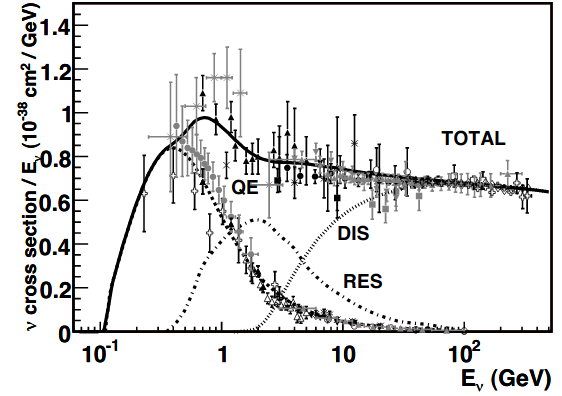
\includegraphics[height=5cm]{diagrams/4-exp/cross_sections_pos.png}%
    }
    \quad
    \subcaptionbox{anti-neutrinos\label{fig:cs_minus}}{%
        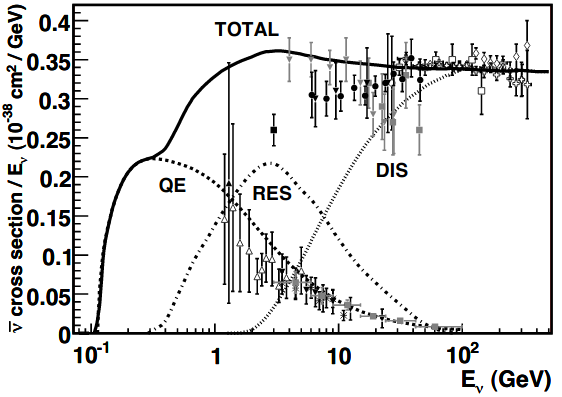
\includegraphics[height=5cm]{diagrams/4-exp/cross_sections_anti.png}%
    }
    \caption[The caption]
    {Figure taken from Ref.\cite{formaggio2012}.}
    \label{fig:cross_sections}
\end{figure}

\begin{figure} % TAU CROSS-SECTION DIAGRAM %
    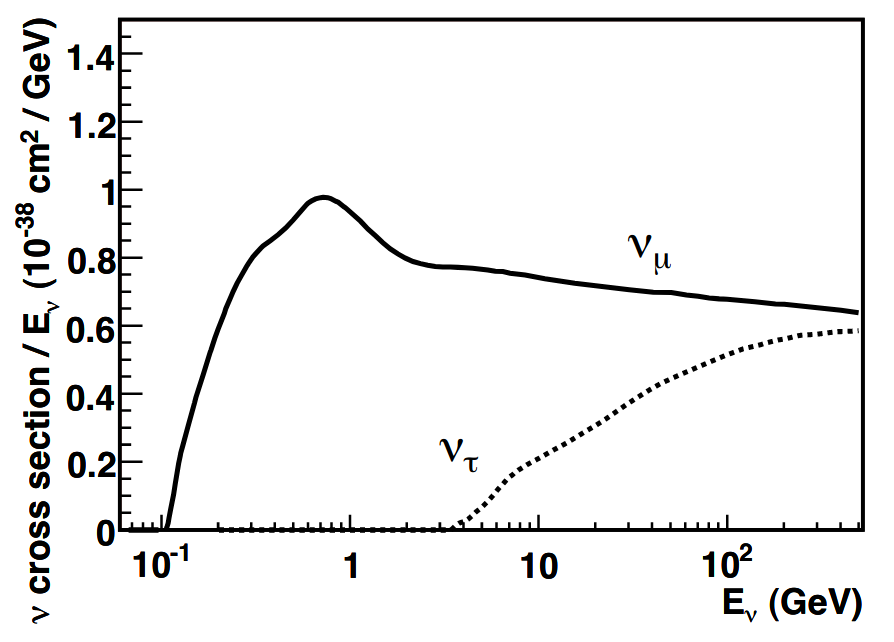
\includegraphics[origin=c,width=0.5\textwidth]{diagrams/4-exp/tau_comparison.png}
    \caption[tau comparison short]
    {Figure taken from Ref.\cite{formaggio2012}.}
    \label{fig:tau_comparison}
\end{figure}

\section{Neutrino experiments} %%%%%%%%%%%%%%%%%%%%%%%%%%%%%%%%%%%%%%%%%%%%%%%%%%%%%%%%%%%%%%%%%%%
\label{sec:exp_exp} %%%%%%%%%%%%%%%%%%%%%%%%%%%%%%%%%%%%%%%%%%%%%%%%%%%%%%%%%%%%%%%%%%%%%%%%%%%%%%

\subsection{The solar sector} %%%%%%%%%%%%%%%%%%%%%%%%%%%%%%%%%%%%%%%%%%%%%%%%%%%%%%%%%%%%%%%%%%%%
\label{sec:exp_exp_solar} %%%%%%%%%%%%%%%%%%%%%%%%%%%%%%%%%%%%%%%%%%%%%%%%%%%%%%%%%%%%%%%%%%%%%%%%

\subsection{The reactor sector} %%%%%%%%%%%%%%%%%%%%%%%%%%%%%%%%%%%%%%%%%%%%%%%%%%%%%%%%%%%%%%%%%%
\label{sec:exp_exp_reactor} %%%%%%%%%%%%%%%%%%%%%%%%%%%%%%%%%%%%%%%%%%%%%%%%%%%%%%%%%%%%%%%%%%%%%%

\subsection{The atmospheric and accelerator sector} %%%%%%%%%%%%%%%%%%%%%%%%%%%%%%%%%%%%%%%%%%%%%%
\label{sec:exp_exp_atmospheric} %%%%%%%%%%%%%%%%%%%%%%%%%%%%%%%%%%%%%%%%%%%%%%%%%%%%%%%%%%%%%%%%%%

\section{Long baseline accelerator water Cherenkov detectors} %%%%%%%%%%%%%%%%%%%%%%%%%%%%%%%%%%%%
\label{sec:exp_long} %%%%%%%%%%%%%%%%%%%%%%%%%%%%%%%%%%%%%%%%%%%%%%%%%%%%%%%%%%%%%%%%%%%%%%%%%%%%%

\subsection{Neutrino beams} %%%%%%%%%%%%%%%%%%%%%%%%%%%%%%%%%%%%%%%%%%%%%%%%%%%%%%%%%%%%%%%%%%%%%%
\label{sec:exp_long_beams} %%%%%%%%%%%%%%%%%%%%%%%%%%%%%%%%%%%%%%%%%%%%%%%%%%%%%%%%%%%%%%%%%%%%%%%

- The Numi beam big paper~\cite{adamson2016}

\begin{figure} % NUMI BEAM DIAGRAM %
    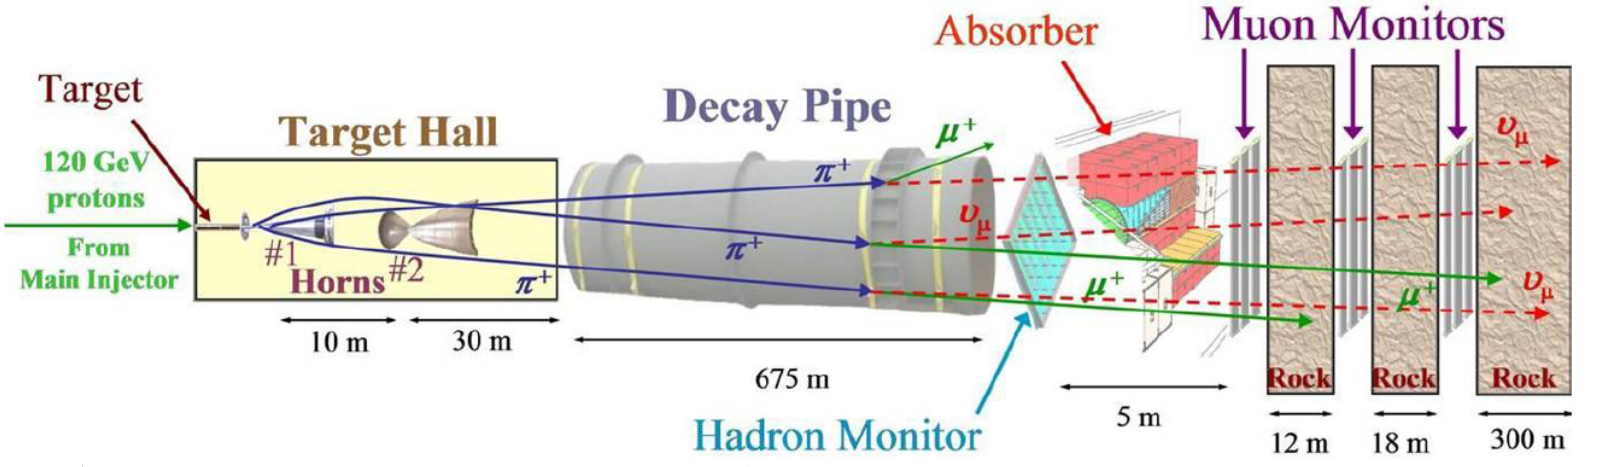
\includegraphics[width=\textwidth]{diagrams/4-exp/numi_beam.png}
    \caption[Schematic of the \numi beam.]
    {Schematic of the main components of the \numi beam (not to scale) shown with their
        dimensions. The horns control if the beam is in neutrino or anti-neutrino mode. Image
        taken from Ref.\cite{adamson2016}.}
    \label{fig:numi_beam}
\end{figure}

\begin{figure} % OFF-AXIS FLUX DIAGRAM %
    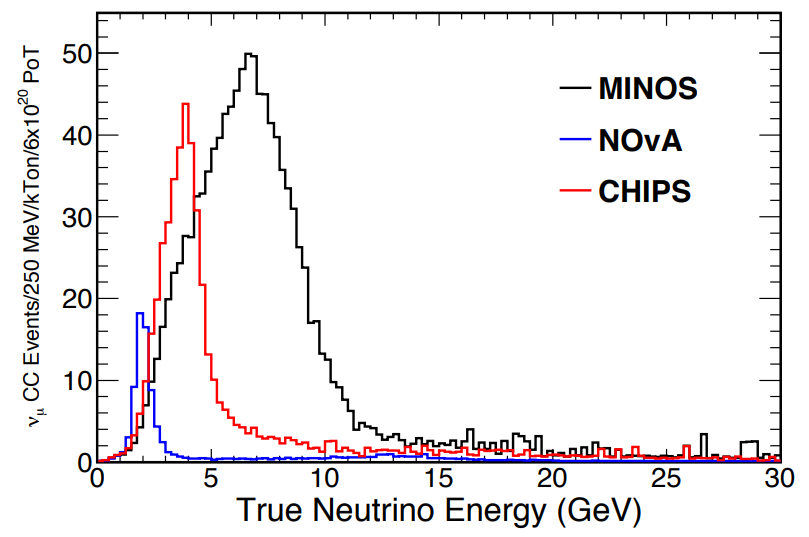
\includegraphics[width=0.6\textwidth]{diagrams/4-exp/numi_axis.png}
    \caption[Neutrino flux for different detectors in the \numi beam.]
    {Neutrino flux for different detectors in the \numi beam.
        The difference is caused by the different off-axis angles.
        Image taken from Ref.\cite{adamson2013}.}
    \label{fig:numi_axis}
\end{figure}

\begin{figure} % CHIPS FLUX DIAGRAM %
    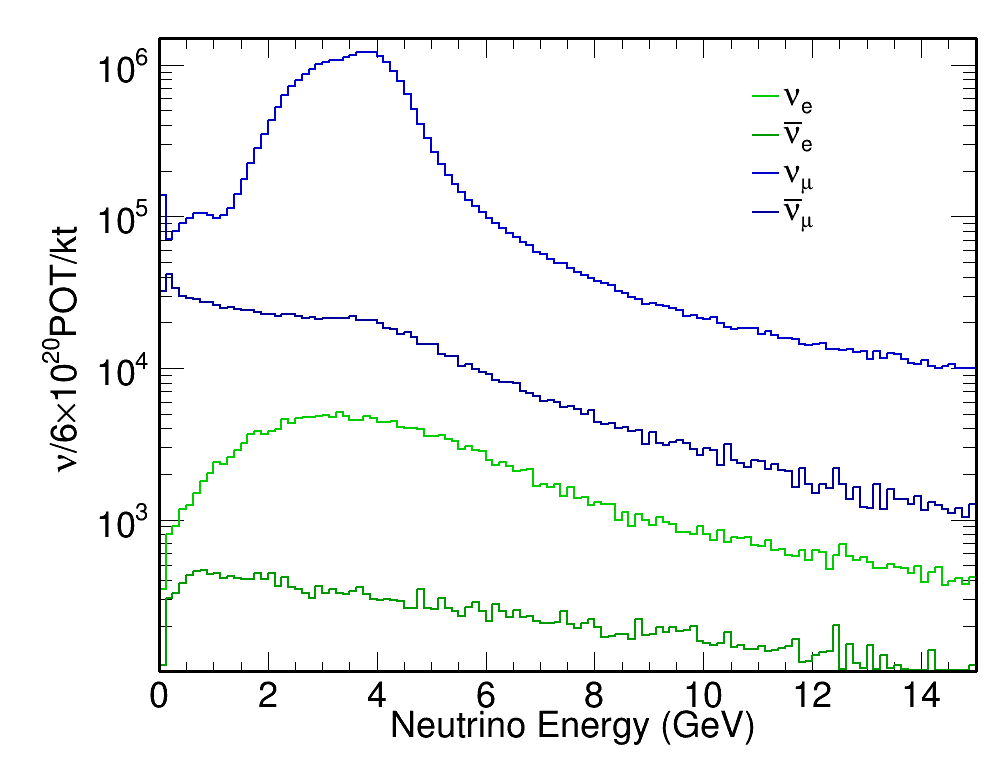
\includegraphics[width=0.6\textwidth]{diagrams/4-exp/flux.png}
    \caption[flux short]
    {}
    \label{fig:flux}
\end{figure}

EQUATION: Off-axis effect equations

\subsection{Cherenkov radiation} %%%%%%%%%%%%%%%%%%%%%%%%%%%%%%%%%%%%%%%%%%%%%%%%%%%%%%%%%%%%%%%%%
\label{sec:exp_long_cherenkov} %%%%%%%%%%%%%%%%%%%%%%%%%%%%%%%%%%%%%%%%%%%%%%%%%%%%%%%%%%%%%%%%%%%

EQUATION: Cherenkov effect equation
DIAGRAM: Cherenkov effect diagram
DIAGRAM: Cherenkov profile diagrams

\subsection{Photomultiplier tubes} %%%%%%%%%%%%%%%%%%%%%%%%%%%%%%%%%%%%%%%%%%%%%%%%%%%%%%%%%%%%%%%
\label{sec:exp_long_pmts} %%%%%%%%%%%%%%%%%%%%%%%%%%%%%%%%%%%%%%%%%%%%%%%%%%%%%%%%%%%%%%%%%%%%%%%%

\section{Future experiments} %%%%%%%%%%%%%%%%%%%%%%%%%%%%%%%%%%%%%%%%%%%%%%%%%%%%%%%%%%%%%%%%%%%%%
\label{sec:exp_future} %%%%%%%%%%%%%%%%%%%%%%%%%%%%%%%%%%%%%%%%%%%%%%%%%%%%%%%%%%%%%%%%%%%%%%%%%%%

Daya bay theta13 Ref.~\cite{an2012}
RENO theta13 Ref.~\cite{ahn2012}
Double Chooz theta13 Ref.~\cite{abe2012}
Hyper-k letter of intent~\cite{abe2011}
Dune CDR~\cite{acciarri2016}

- With the measurements of a non-zero theta13 by reactor neutrino experiments, the main focus now
has shifted to resolving the mass hierarchy ambiguity and measuring delta-cp. These can be probed
by long-baseline neutrino experiments by looking to numu to nuel transitions.
- BIG EQUATION FOR PROBABILITY: shows sensitivity to the mass hiearchy through the matter effect
parameters A and to the cp-violtating phase trhough the second term.
- Over that last 20 years neutrino oscillations have become well-established and we are now moving
into the precision measurement era.
- DUNE is a next-generation neutrino oscillation experiment with a primary scientific goal of
observation of CP-violation in the neutrino sector.
- In DUNE a muon neutrino(anti-neutrino) beam will be produced by the Long-Baseline Neutrino
Facility (LBNF)
- There will be a near detector at Fermilab before the neutrinos travel the 1285km to the Sanford
Underground Research Facility (SURF) in South Dakota.
- The far detector will consist of four 10kt (fiducial) liquid argon time projections chamber
(LArTPC) detectors.
- Neutrino oscillation probabilities can then be infered by comparisons of the observed neutrino
spectra and the near and far detectors.
- Recent obsevation of a large theta13 have focuseed the next genetation of long baseline
experiments towards the mass hierarchy, octant of theta23 and measureing delta-CP
- Nova and T2k will not be able to measure the remaining unknows (check this)
- Dune will hopefully solve these problems but will be increadibly expensive

- Symmetries under charge-conjugation and parity inversion are both macimally violated by the
waek interaction.
- Their combined operation has been shown to be violated, to a small degress, by quark mixing
processes.
- If sin(delta-cp) is non zero then vacuum oscillation properties of nu and anti nu will be
different.
- DUNE (I assume CHIPS) is sensative to four oscillation paramters, delta31, theta23, theta13
and delta-cp.
- These can be measured using four data sample, two for neutrino and two for antineutrinos.
- These sample are produced by "Forward Horn current" FHC and "Reverse Horn current" RHC,
producing predominetetly neutrinos and anti-neutrinos respectively.
- Dissapearence channels sensitive to %abs(delta31^2), and sin^2(2theta23).
- Apperence channels sensitive to all four parameters including sign of %delta32^2.
- The "signal" in all cases are CC interactions, therefore selection of nuel, anuel, numu and
anumu CC is the goal.
- Main background in CC numu selections are NC with charged pions.
- Main background in CC nuel selections is pi-zero NC, which can mimic the chracteristic EM
shower, due to its near certain decay into two photons.
- You get a small number of nuel intrinsic to the beam, they are just a background as they are
indistinguishabe from the nuel appreaence neutrinos.
- Once you have collected samples in all four cases, a fit is performed to the reconstructed
neutrino energy distributions to extract the four neutrino oscillation parameters.